%%%%%%%%%%%%%%%%%%%%%%%%%%%%%%%%%%%%%%%%%%%%%%%%%%%%%%%%%%%%%%%%%
% Desde el terminal 
% xelatex docencia.tex
% MUW Presentation
% LaTeX Template
% Version 1.0 (27/12/2016)
%
% License:
% CC BY-NC-SA 4.0 (http://creativecommons.org/licenses/by-nc-sa/3.0/)
%
% Created by:
% Nicolas Ballarini, CeMSIIS, Medical University of Vienna
% nicoballarini@gmail.com
% http://statistics.msi.meduniwien.ac.at/
%
% Customized for UAH by:
% David F. Barrero, Departamento de Automática, UAH
%%%%%%%%%%%%%%%%%%%%%%%%%%%%%%%%%%%%%%%%%%%%%%%%%%%%%%%%%%%%%%%%%

\documentclass[10pt,compress]{beamer} % Change 10pt to make fonts of a different size
\mode<presentation>

\usepackage[spanish]{babel}
\usepackage{fontspec}
\usepackage{tikz}
\usepackage{etoolbox}
\usepackage{listings}

% Custom packages
\usepackage{tabularx}
\usepackage{booktabs}
\usepackage{standalone}
\usepackage{pgfpages}
\usetikzlibrary{arrows,positioning,backgrounds,intersections,calc,snakes}

%\setbeameroption{show notes on second screen}

\usetheme{UAH}
\usecolortheme{UAH}
\setbeamertemplate{navigation symbols}{} 
\setbeamertemplate{caption}[numbered]

%%%%%%%%%%%%%%%%%%%%%%%%%%%%%%%%%%%%%%%%%%%%%%%%%%%%%%%%%%%%%%%%%
%% Presentation Info
\title[Grupo de Sistemas Inteligentes]{Grupo de Sistemas Inteligentes}
\author{Departamento de Automática}
\institute{Universidad de Alcalá}
\date{Dr. David Fernández Barrero}
%%%%%%%%%%%%%%%%%%%%%%%%%%%%%%%%%%%%%%%%%%%%%%%%%%%%%%%%%%%%%%%%%


%%%%%%%%%%%%%%%%%%%%%%%%%%%%%%%%%%%%%%%%%%%%%%%%%%%%%%%%%%%%%%%%%
%% Descomentar para habilitar barra de navegación superior
%% \setNavigation
%%%%%%%%%%%%%%%%%%%%%%%%%%%%%%%%%%%%%%%%%%%%%%%%%%%%%%%%%%%%%%%%%

%%%%%%%%%%%%%%%%%%%%%%%%%%%%%%%%%%%%%%%%%%%%%%%%%%%%%%%%%%%%%%%%%
%% Configuración de logotipos en portada
%% Opacidad de los logotipos
\newcommand{\opacidad}{1}
%% Descomentar para habilitar logotipo en pié de página de portada
\renewcommand{\logoUno}{Images/isg.png}
%% Descomentar para habilitar logotipo en pié de página de portada
%\renewcommand{\logoDos}{Images/CCLogo.png}
%% Descomentar para habilitar logotipo en pié de página de portada
%\renewcommand{\logoTres}{Images/ALogo.png}
%% Descomentar para habilitar logotipo en pié de página de portada
%\renewcommand{\logoCuatro}{Images/ELogo.png}
%%%%%%%%%%%%%%%%%%%%%%%%%%%%%%%%%%%%%%%%%%%%%%%%%%%%%%%%%%%%%%%%%

%%%%%%%%%%%%%%%%%%%%%%%%%%%%%%%%%%%%%%%%%%%%%%%%%%%%%%%%%%%%%%%%%
%% FOOTLINE
%% Comment/Uncomment the following blocks to modify the footline
%% content in the body slides. 


%% Option A: Title and institute
\footlineA
%% Option B: Author and institute
%\footlineB
%% Option C: Title, Author and institute
%\footlineC
%%%%%%%%%%%%%%%%%%%%%%%%%%%%%%%%%%%%%%%%%%%%%%%%%%%%%%%%%%%%%%%%%

\begin{document}

%%%%%%%%%%%%%%%%%%%%%%%%%%%%%%%%%%%%%%%%%%%%%%%%%%%%%%%%%%%%%%%%%
% Use this block for a blue title slide with modified footline
{\titlepageBlue
	% Content
    \begin{frame}
        \titlepage
    \end{frame}
}

%\begin{frame}{Plaza}

%\color{azulUAH}

%\noindent {\sc Cuerpo}: Profesor Titular de Universidad

%\noindent {\sc Departamento}: Automática

%\noindent {\sc Área de Conocimiento}: Arquitectura y Tecnología de Computadores

%\noindent {\sc Perfil Docente}: \textbf{Sistemas Operativos (Grado de Ingeniería Informática y Grado en Ingeniería de Computadores)}

%\noindent {\sc Perfil Investigador}: Mejora de la gestión de recursos hospitalarios mediante predicción de la demanda con Aprendizaje Automático y Optimización

%\noindent {\sc Código de la Plaza}: Z029/DAQ208

%\noindent {\sc BOE}: 5 de mayo de 2018

    %%%%%%%%%%%%%%%%%%%%%%%%%%% COMENTARIOS %%%%%%%%%%%%%%
%        \note{
%}
%\end{frame}

\institute{Presentación Grupo de Sistemas Inteligentes}

%%%%%%%%%%%%%%%%%%%%%%%%%%%%%%%%%%%%%%%%%%%%%%%%%%%%%%%%%%%%%%%%%
% Comment/Uncomment these lines for an automatically generated outline.
{\disableNavigation{white}
    \begin{frame}{Índice}
        \tableofcontents
    \end{frame}
      %%%%%%%%%%%%%%%%%%%%%%%%%%% COMENTARIOS %%%%%%%%%%%%%%
    \note {    
   Esta parte la he dividido en 3 partes: comienzo con un contexto de la docencia en la UAH, 
   a continuación describo el proyecto docente,  y finalizo con la metodología docente aplicable de 2 de los proyectos de 
   innovación en los que he participado.
  
   \tableofcontents
   }
}

\addtocounter{framenumber}{-1} %To control the number in which numbering begins

%%%%%%%%%%%%%%%%%%%%%%%%%%%%%%%%%%%%%%%%%%%%%%%%%%%%%%%%%%%%%%%%%
\section{La Universidad de Alcalá}
{
    \sectionheaderWhite %Enclose the frame with {} and add this command for white background in section header
    \begin{frame}{La Universidad de Alcalá}{Contexto institucional}
    \end{frame}
}

\subsection{Universidad de Alcalá}

\begin{frame}{Universidad de Alcalá}
    \begin{columns}
         \column{.05\textwidth}
         \column{.60\textwidth}
         Historia
        \begin{itemize}
            \item Fundada en 1499
            \item Trasladada a Madrid en 1836
            \item Refundada en 1977
        \end{itemize}
        Estructura
        \begin{itemize}
            \item 3 campus
            \item 23 departamentos, 7 facultades, 3 escuelas
        \end{itemize}
        Capital humano
        \begin{itemize}
            \item 28.128 alumnos (grado + postgrado)
            \item 1.662 PDI + 790 PAS
        \end{itemize}
        Oferta académica
        \begin{itemize}
            \item 38 grados, 49 másteres
        \end{itemize}
         \column{.30\textwidth}
            
\includegraphics[width=\linewidth]{figs/03_logo-vC_pant293.pdf}\\
            \bigskip
            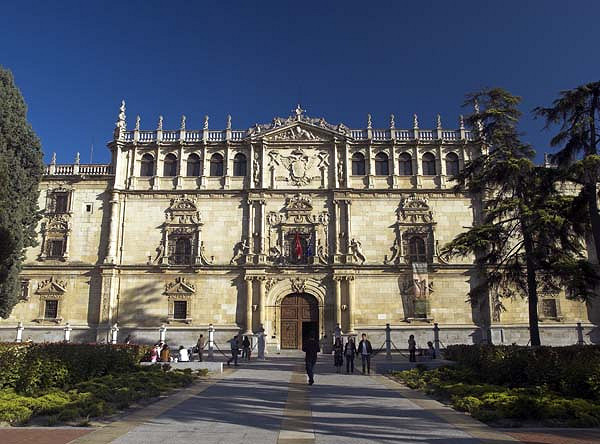
\includegraphics[width=\linewidth]{figs/fachada}\\
         \column{.05\textwidth}
    \end{columns}
         %%%%%%%%%%%%%%%%%%%%%%%%%%% COMENTARIOS %%%%%%%%%%%%%%
        \note{
       \begin{itemize}
        \item  La antigua UAH, conocida también como universidad Complutense tuvo una larga vida (1499-1836), fecha 
        que se trasladó a Madrid. Fue Refundada en 1977.
        \item UAH está DIVIDIDA en tres grandes unidades físicas\\
		- Campus de Alcalá Ciudad (CAC): Facultades de letras, económicas, empresariales y Turismo y arquitectura\\
		- Camp Universitario (CUn): CC de la Salud, CC Experimentales y la EPS (con los grados de Ingeniería 
		Telecomunicaciones, Informática e Industriales) \\
		-  Cam de Guadalajara (CG): Facul de Educación, Turismo, Administración y Dirección de Empresas, CC 
		y Tecnología de la Edificación,  Enfermería y Comunic. Audiovisual.  \\
        \item 23 departamentos, 7 facultades, 3 escuelas
        \begin{itemize}
           \item EL NUMERO DE ALUMNOS MATRICULADOS en el curso 2016-17 es de algo más de 28.000, de los cuales la 
           mitad 14228) son estudiantes de grado en centros propios, más de 1000 alumnos de grado en centros adscritos, 
           y EL RESTO pertenecen a postgrado. $28.128$ alumnos (grado + postgrado)
            \item EN CUANTO a PDI, la proporción es 60\% H, y 40\% M, $1.662$ PDI ($986$H + $676$M)
            \item EN CAMBIO en PAS, la proporción es 37\% H y 43\%M  $790$ PAS ($290$H + $500$M)
        \end{itemize}
        \end{itemize}
        }
\end{frame}

\subsection{Escuela Politécnica Superior}

\begin{frame}{La Universidad de Alcalá}{Escuela Politécnica Superior}

    \centering Alumnos matriculados en la EPS por grado
    \vspace{-0.6cm}

     \begin{table}
       \begin{tabularx}{0.85\textwidth}	{Xc}\\  \toprule %{0.6\textwidth}{Xc}	\toprule
         \sc{Grado} &  \sc{Alumnos} \\ \midrule
        Grado en Ing. en Electrónica y Automática Industrial & 416 \\ 
        Grado en Ing. Electrónica de Comunicaciones & 246 \\ 
        Grado en Ing. en Sist. de Telecomunicación  & 221 \\ 
        Grado en Ing. en Tecnologías de Telecomunicación & 240 \\
        Grado en Ing. Telemática           & 189 \\  
        Grado en Ing. Informática          & 350 \\ 
        Grado en Ing. de Computadores      & 245 \\ 
        Grado en Sistemas de Información   & 302 \\ \midrule
        Total                              & 2.209 \\ \bottomrule
    \end{tabularx}

    %Planes de estudio de máster

    %\begin{itemize}
    %    \item Máster Universitario en Ingeniería en Telecomunicación especialidad Tecnologías Espaciales y de Defensa
    %    \item Máster Universitario en Analítica de Negocio y Grandes Volúmenes de Datos
    %\end{itemize}

 \end{table}
    %%%%%%%%%%%%%%%%%%%%%%%%%%% COMENTARIOS %%%%%%%%%%%%%%
    \note{   
    }
\end{frame}

\section{Grupo de Sistemas Inteligentes}
{
    \sectionheaderWhite %Enclose the frame with {} and add this command for white background in section header
    \begin{frame}{Grupo de Sistemas Inteligentes}{Personal, áreas de investigación y proyectos}
    \end{frame}
}

\subsection{Personal}
\begin{frame}{Grupo de Sistemas Inteligentes}{Personal}
    \begin{columns}
         \column{.60\textwidth}
    Grupo multidisciplinar fundado en 2008
        \begin{itemize}
        \item Directora: Dra. Mª Dolores Rodríguez
		%\item Inteligencia Artificial aplicada
        \item Departamentos de Automática y Ciencias de la Computación
        \end{itemize}

	Personal GSI
		\begin{itemize}
		\item Una catedrática
		\item Tres profesores titulares
		\item Dos colaboradores doctores
		\end{itemize}

    \column{.40\textwidth}
		
\includegraphics[width=\textwidth]{figs/isg-color}\\
		\smallskip
	 	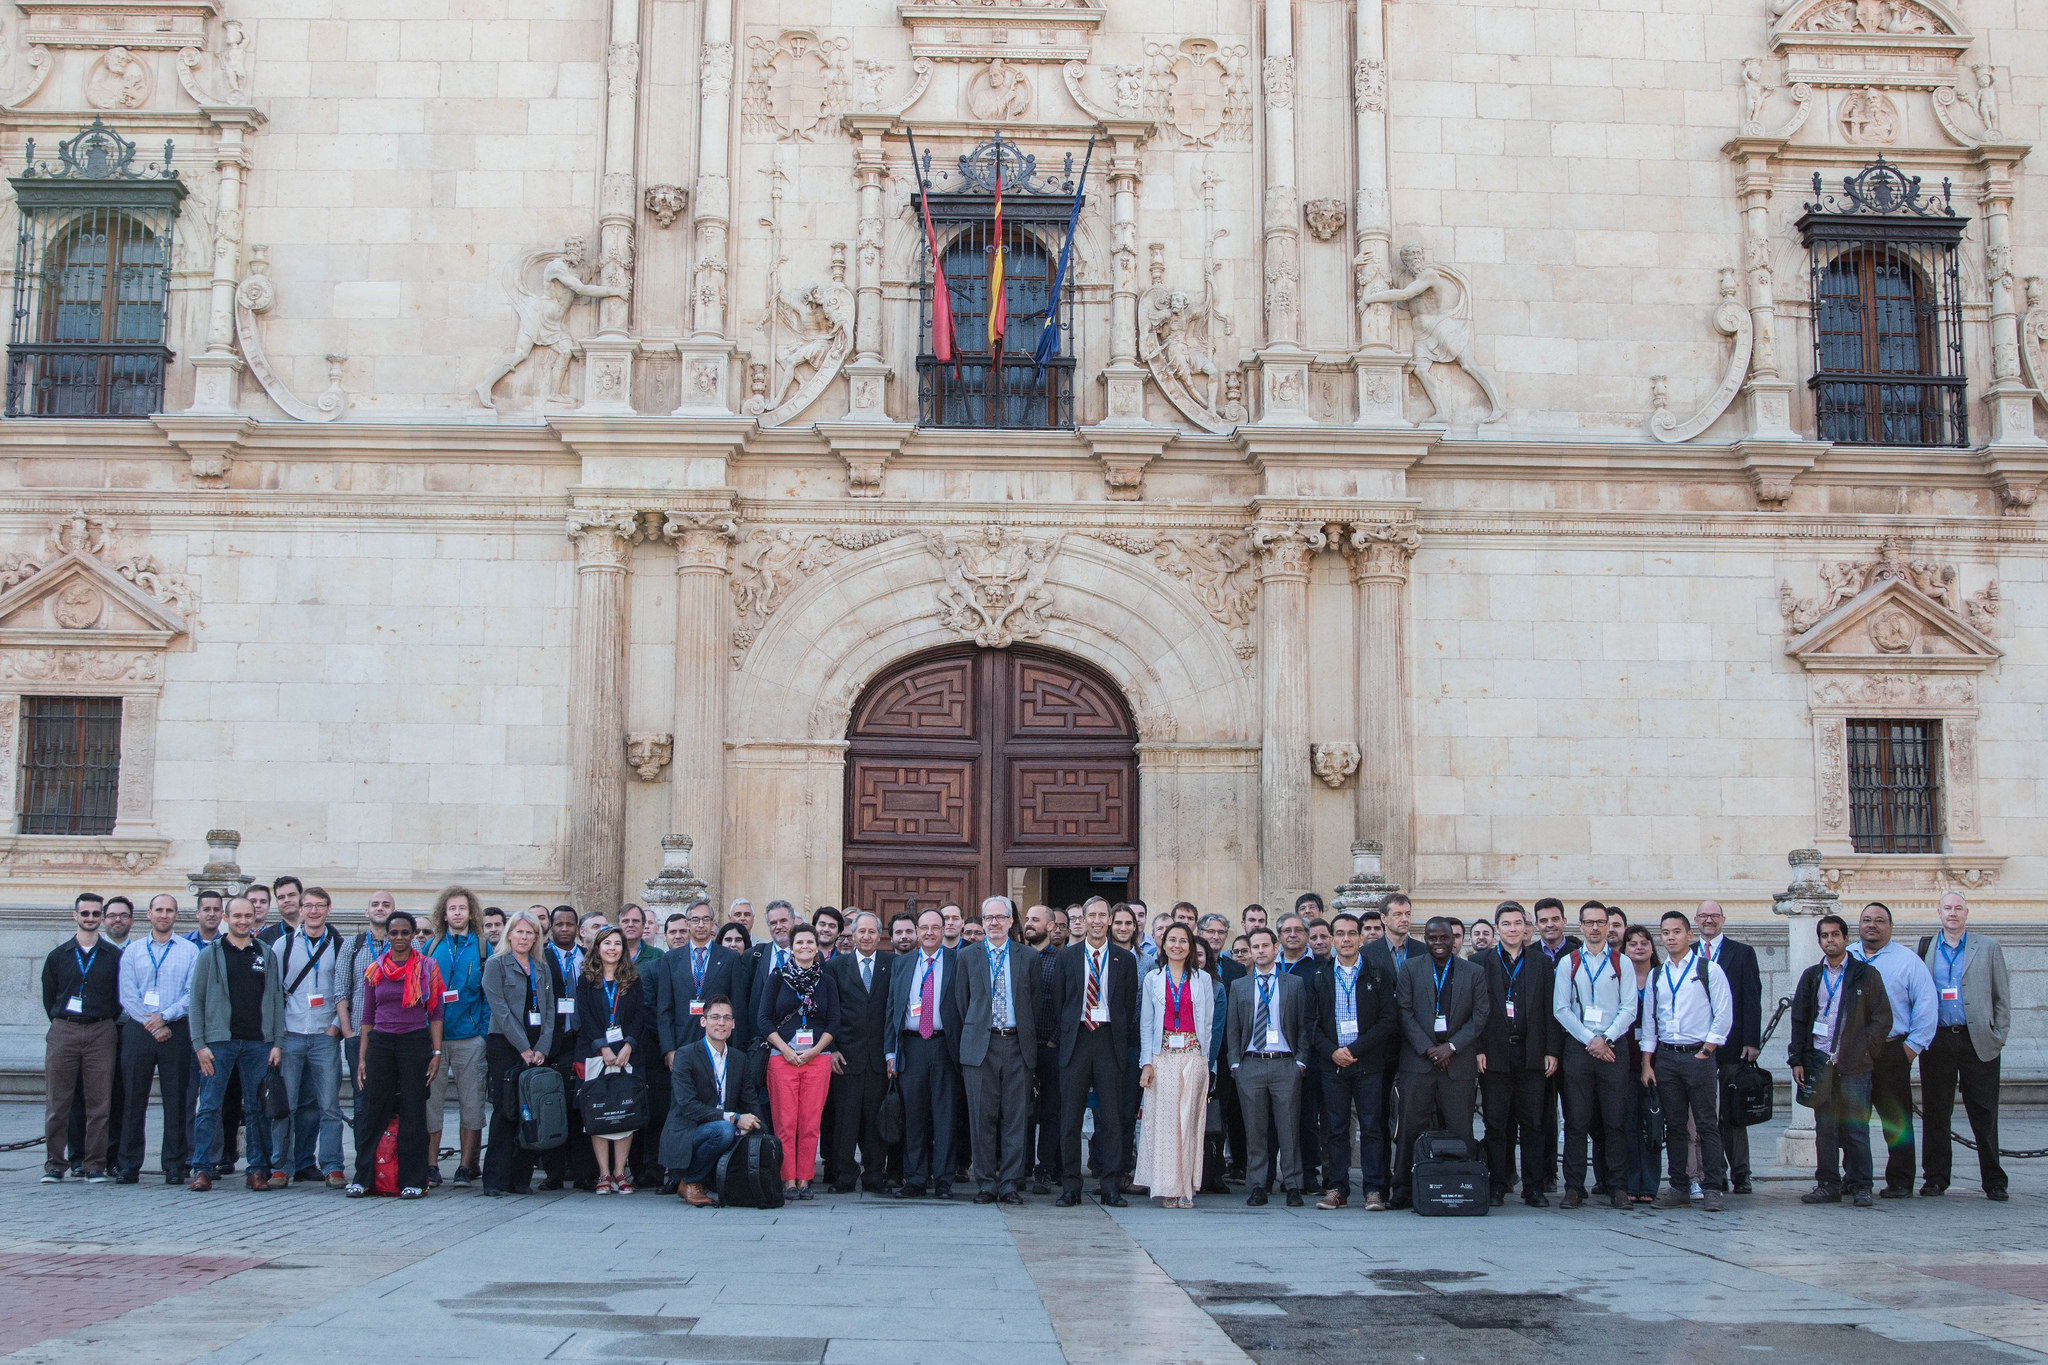
\includegraphics[width=\textwidth]{figs/smcit}
    \end{columns}

    %%%%%%%%%%%%%%%%%%%%%%%%%%% COMENTARIOS %%%%%%%%%%%%%%    
    \note{    
    }
\end{frame}

\subsection{Áreas de investigación}
\begin{frame}{Grupo de Sistemas Inteligentes}{Áreas de investigación}
    \begin{columns}
         \column{.60\textwidth}
    		Investigación en Inteligencia Artificial aplicada
    		\begin{itemize}
        		\item Planificación y optimización de tareas y rutas
        		\item Control autónomo
        		\item Aprendizaje Automático
        		\item Computación bioinspirada
        	\end{itemize}

    		Dominios de aplicación
        	\begin{itemize}
        		\item Ingeniería espacial
        		\item Seguridad
        		\item \textit{eHealth}
        	\end{itemize}
        
         \column{.40\textwidth}
	 		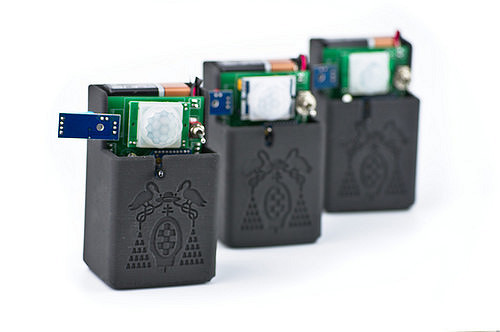
\includegraphics[width=\textwidth]{figs/sensores}\\
	 		%\centering 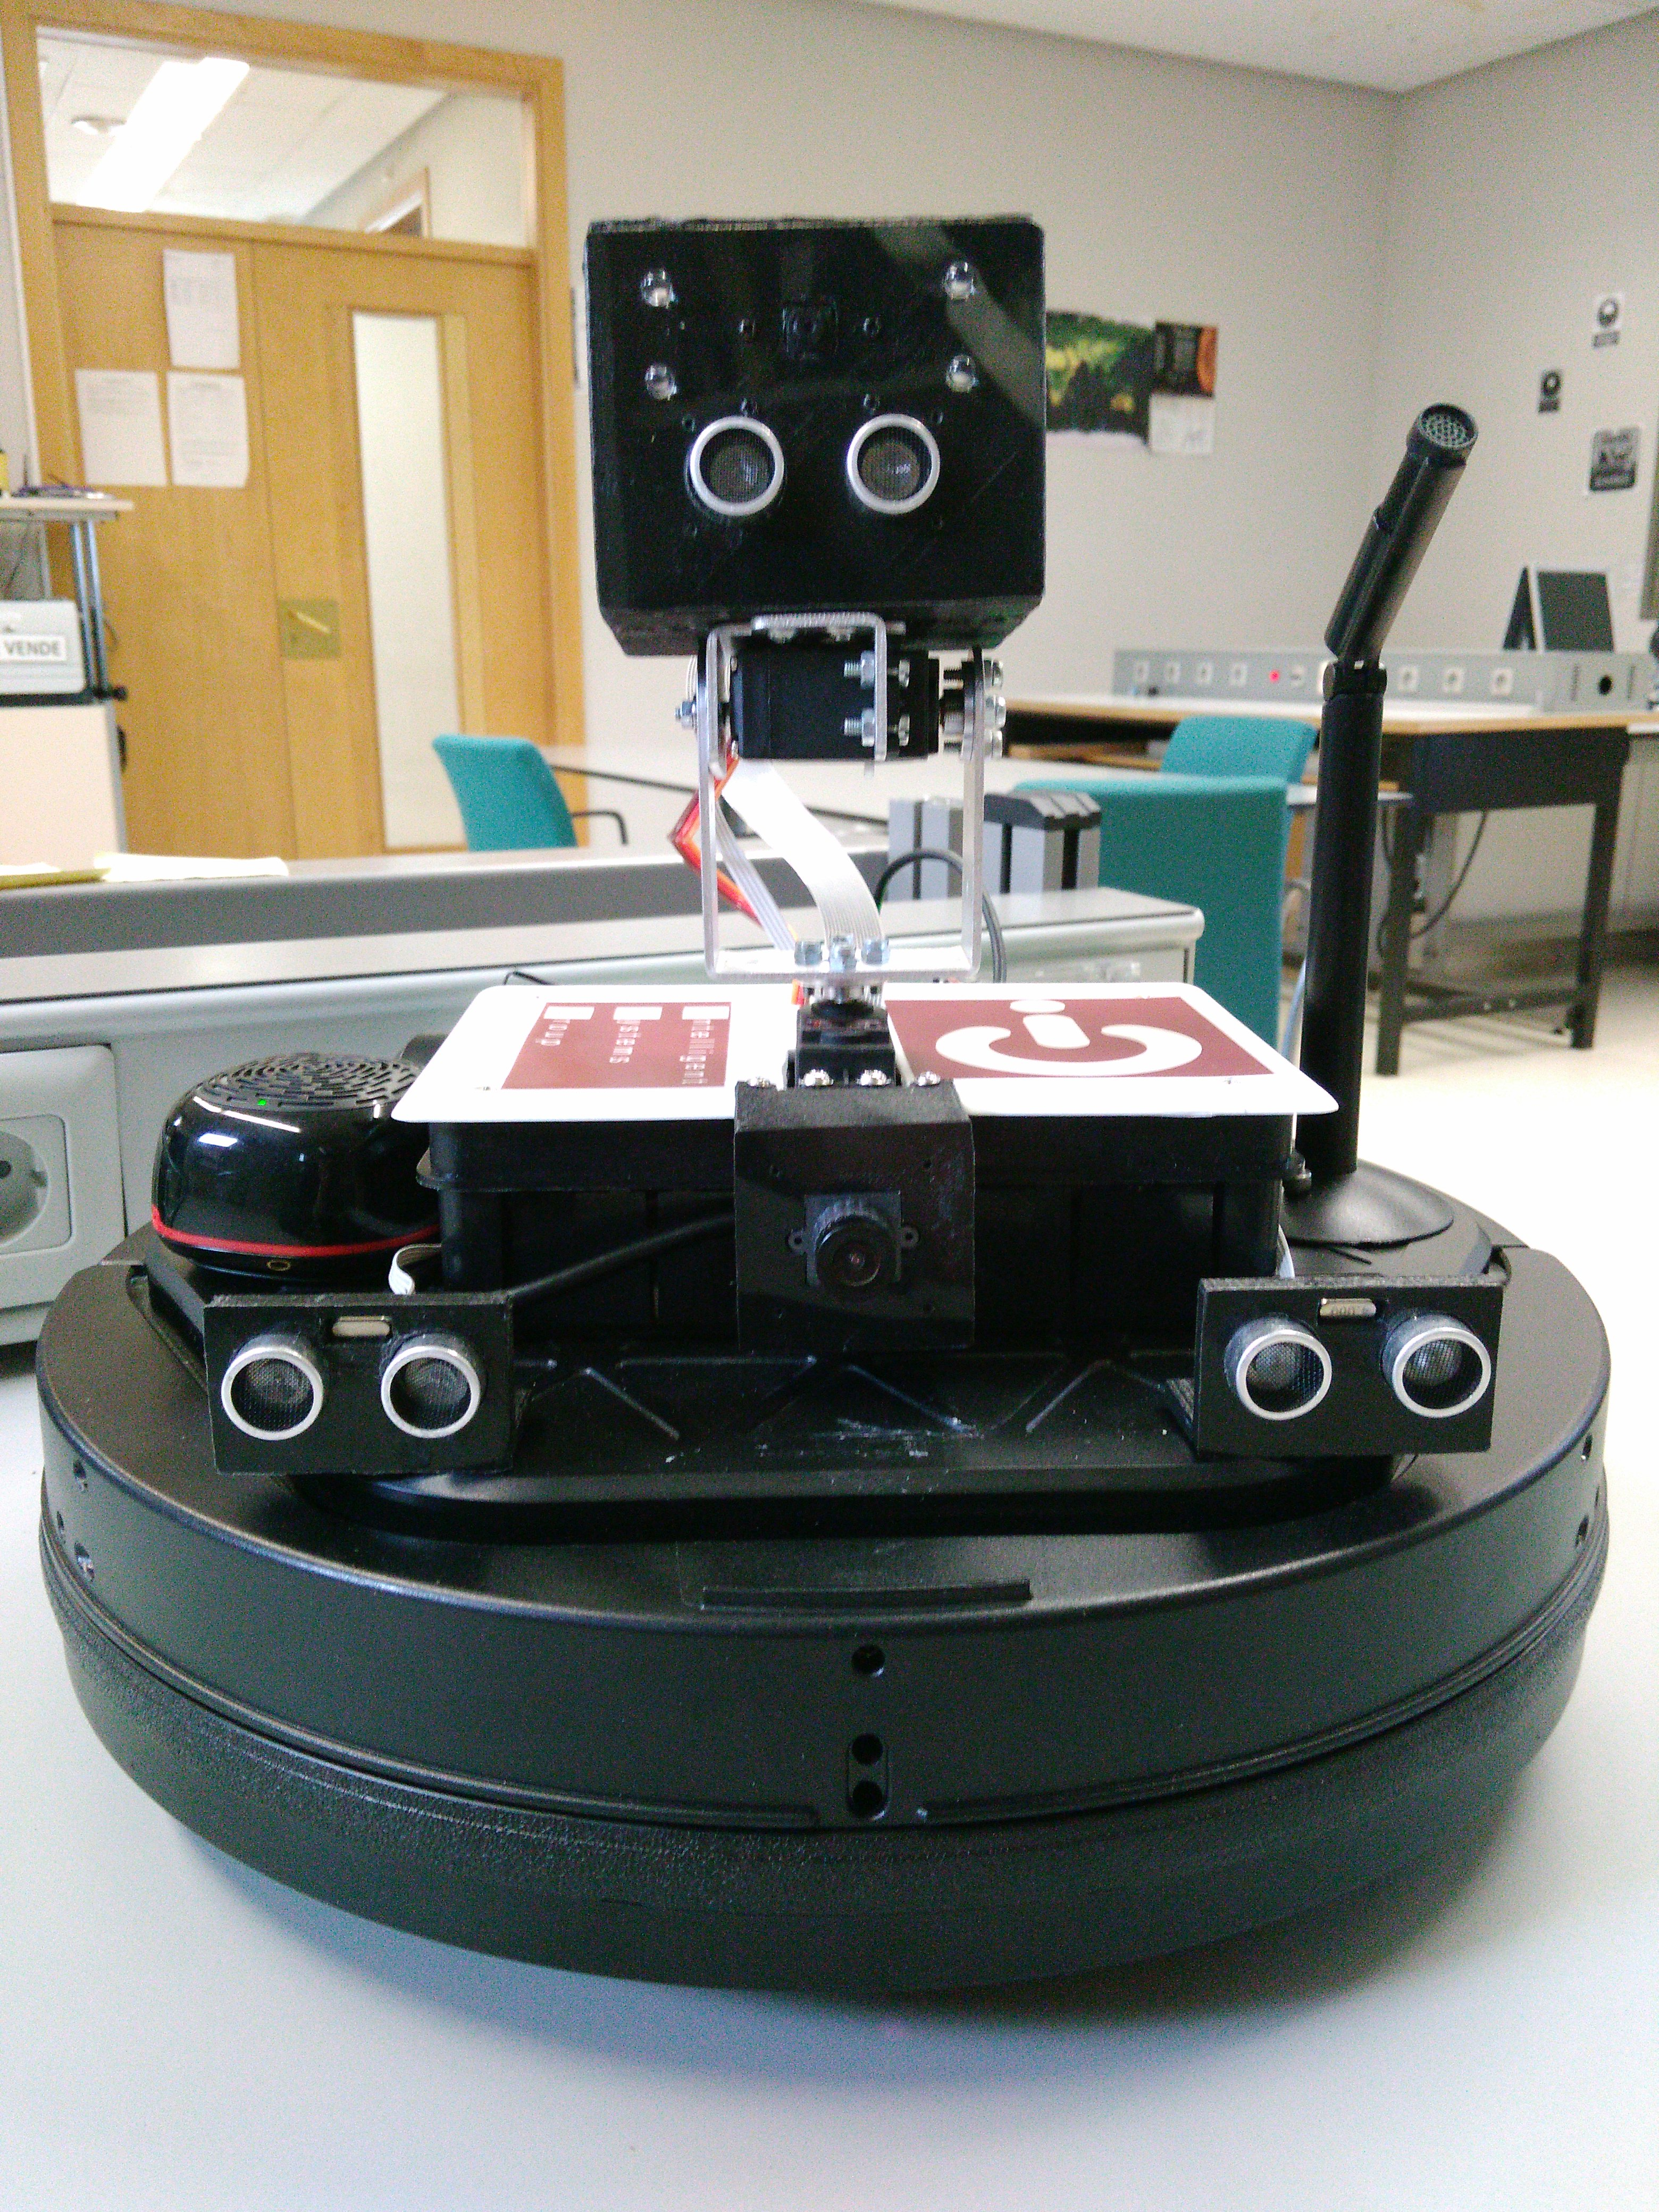
\includegraphics[width=0.7\textwidth]{figs/robot}
	\end{columns}
     %%%%%%%%%%%%%%%%%%%%%%%%%%% COMENTARIOS %%%%%%%%%%%%%%    
    \note{    
    }
\end{frame}

\subsection{Proyectos}
\begin{frame}{Grupo de Sistemas Inteligentes}{Proyectos (I)}
    Proyectos ESA
        \begin{itemize}
            \item \textit{Cooperative systems for autonomous exploration missions}
            \item \textit{Autonomy for interplanetary missions}
            \item \textit{Advanced Mission Operations Concepts \& Technologies for Future ESA Missions}
        \end{itemize}
    Proyectos empresas
        \begin{itemize}
        \item \textit{SAVIERX2: Demostrador de tecnologías de interacción hombre-máquina con UAS} - AIRBUS
        \item \textit{COLlaborative Vehicles autonomous EXploration System (COLVEX)} - IXION
        \end{itemize}

	 Convenios
        \begin{itemize}
            \item NASA - \textit{Jet Propulsion Laboratory}
        \end{itemize}
    
     \smallskip 
     \centering

    
\includegraphics[height=25pt]{figs/esalogo}
    \quad
    
\includegraphics[height=20pt]{figs/ixionlogo}
    \quad
    
\includegraphics[height=30pt]{figs/airbuslogo}     
    %\quad
    %
\includegraphics[height=25pt]{figs/jpllogo}
    \quad
    
\includegraphics[height=25pt]{figs/NASA}

%%%%%%%%%%%%%%%%%%%%%%%%%%% COMENTARIOS %%%%%%%%%%%%%%    
    \note{
    }  
\end{frame}


\begin{frame}{Grupo de Sistemas Inteligentes}{Proyectos (II)}
    Proyectos Aprendizaje Automático
        \begin{itemize}
            \item \textit{Detección de defectos de fabricación en perfiles de PVC}. Profine Iberia
            \item \textit{Detección de caídas mediante acelerómetro triaxial en entornos de atención a la dependencia}. UAH
            \item \textit{Detección automática de emergencias basada en patrones de conducta en personas dependientes}. UAH
        \end{itemize}
    
    \begin{columns}
         \column{.50\textwidth}
             \begin{block}{Resumen proyectos}
                \begin{itemize}
                \item 32 proyectos nacionales
                \item 12 proyectos internacionales
              \end{itemize}
             \end{block}
         \column{.50\textwidth}
              \begin{block}{Resumen publicaciones}
                \begin{itemize}
                \item 40 revistas y capítulos libro
                \item 74 conferencias
              \end{itemize}
             \end{block}
    \end{columns}

%%%%%%%%%%%%%%%%%%%%%%%%%%% COMENTARIOS %%%%%%%%%%%%%%    
    \note{
    }  
\end{frame}

%\section*{}
{
    \sectionheaderWhite %Enclose the frame with {} and add this command for green background in section header
    \begin{frame}[plain]{Gracias por su atención}{Dr. David Fernández Barrero}
    \small{
    %Libro: \LaTeX, plantilla \textit{classicthesis}\\
    Presentación: Beamer\\
    Imágenes: Ti\emph{k}z\\
    Gráficos: R/Lattice
    }
    \end{frame}
    \note{
    GRACIAS POR SU ATENCIÓN, Y QUEDO A LA DISPOSICIÓN DEL TRIBUNAL PARA CUALQUIER PREGUNTA QUE QUIERAN HACERME}
}

\institute{Departamento de Automática}
\title{Grupo de Sistemas Inteligentes}
\author{Departamento de Automática}
\institute{Universidad de Alcalá}
\date{Dr. David Fernández Barrero}
%
{\titlepageBlue
	% Content
    \begin{frame}
        \titlepage
        \note{Sr. PRESIDENTE, SRS. MIEMBROS de la comisión, señores y señoras, Buenos días\\. 
	          }
    \end{frame}
}

\end{document}
